\documentclass[12pt,english,french]{article}\usepackage{graphicx, color}
%% maxwidth is the original width if it is less than linewidth
%% otherwise use linewidth (to make sure the graphics do not exceed the margin)
\makeatletter
\def\maxwidth{ %
  \ifdim\Gin@nat@width>\linewidth
    \linewidth
  \else
    \Gin@nat@width
  \fi
}
\makeatother

\IfFileExists{upquote.sty}{\usepackage{upquote}}{}
\definecolor{fgcolor}{rgb}{0.2, 0.2, 0.2}
\newcommand{\hlnumber}[1]{\textcolor[rgb]{0,0,0}{#1}}%
\newcommand{\hlfunctioncall}[1]{\textcolor[rgb]{0.501960784313725,0,0.329411764705882}{\textbf{#1}}}%
\newcommand{\hlstring}[1]{\textcolor[rgb]{0.6,0.6,1}{#1}}%
\newcommand{\hlkeyword}[1]{\textcolor[rgb]{0,0,0}{\textbf{#1}}}%
\newcommand{\hlargument}[1]{\textcolor[rgb]{0.690196078431373,0.250980392156863,0.0196078431372549}{#1}}%
\newcommand{\hlcomment}[1]{\textcolor[rgb]{0.180392156862745,0.6,0.341176470588235}{#1}}%
\newcommand{\hlroxygencomment}[1]{\textcolor[rgb]{0.43921568627451,0.47843137254902,0.701960784313725}{#1}}%
\newcommand{\hlformalargs}[1]{\textcolor[rgb]{0.690196078431373,0.250980392156863,0.0196078431372549}{#1}}%
\newcommand{\hleqformalargs}[1]{\textcolor[rgb]{0.690196078431373,0.250980392156863,0.0196078431372549}{#1}}%
\newcommand{\hlassignement}[1]{\textcolor[rgb]{0,0,0}{\textbf{#1}}}%
\newcommand{\hlpackage}[1]{\textcolor[rgb]{0.588235294117647,0.709803921568627,0.145098039215686}{#1}}%
\newcommand{\hlslot}[1]{\textit{#1}}%
\newcommand{\hlsymbol}[1]{\textcolor[rgb]{0,0,0}{#1}}%
\newcommand{\hlprompt}[1]{\textcolor[rgb]{0.2,0.2,0.2}{#1}}%

\usepackage{framed}
\makeatletter
\newenvironment{kframe}{%
 \def\at@end@of@kframe{}%
 \ifinner\ifhmode%
  \def\at@end@of@kframe{\end{minipage}}%
  \begin{minipage}{\columnwidth}%
 \fi\fi%
 \def\FrameCommand##1{\hskip\@totalleftmargin \hskip-\fboxsep
 \colorbox{shadecolor}{##1}\hskip-\fboxsep
     % There is no \\@totalrightmargin, so:
     \hskip-\linewidth \hskip-\@totalleftmargin \hskip\columnwidth}%
 \MakeFramed {\advance\hsize-\width
   \@totalleftmargin\z@ \linewidth\hsize
   \@setminipage}}%
 {\par\unskip\endMakeFramed%
 \at@end@of@kframe}
\makeatother

\definecolor{shadecolor}{rgb}{.97, .97, .97}
\definecolor{messagecolor}{rgb}{0, 0, 0}
\definecolor{warningcolor}{rgb}{1, 0, 1}
\definecolor{errorcolor}{rgb}{1, 0, 0}
\newenvironment{knitrout}{}{} % an empty environment to be redefined in TeX

\usepackage{alltt}
\usepackage[francais]{babel}
\usepackage[T1]{fontenc}
\usepackage{lmodern}
\usepackage[utf8]{inputenc}
\usepackage{numprint}
\usepackage{url}
\usepackage{makeidx}
\makeindex



\begin{document}

\title{CESU - Travail Véronique Brunstein}
\author{V.Brunstein and JCB}
\date{\today}
\maketitle

\section{Les données}

\begin{knitrout}
\definecolor{shadecolor}{rgb}{0.969, 0.969, 0.969}\color{fgcolor}\begin{kframe}
\begin{verbatim}
##  [1] "X"                                                                  
##  [2] "Groupe"                                                             
##  [3] "date"                                                               
##  [4] "Numéro"                                                             
##  [5] "Diplôme"                                                            
##  [6] "Date"                                                               
##  [7] "Sexe"                                                               
##  [8] "Lieu.exercice"                                                      
##  [9] "experience.urgence.1...oui.2...non"                                 
## [10] "Date.debut"                                                         
## [11] "date.fin"                                                           
## [12] "confronté.situation.jamais...1.rarement...2.parfois...3.souvent...4"
## [13] "de.quand.date.dernière.situation.d.urgence"                         
## [14] "de.quand.date.dernière.situation.d.urgence.1"                       
## [15] "formation.urgence"                                                  
## [16] "date.derniere.formation.urgence"                                    
## [17] "date.derniere.formation.urgence.1"                                  
## [18] "A"                                                                  
## [19] "B"                                                                  
## [20] "C"                                                                  
## [21] "D"                                                                  
## [22] "E"                                                                  
## [23] "F"                                                                  
## [24] "G"                                                                  
## [25] "H"                                                                  
## [26] "I"                                                                  
## [27] "J"                                                                  
## [28] "K"                                                                  
## [29] "L"                                                                  
## [30] "M"                                                                  
## [31] "N"                                                                  
## [32] "Q1A"                                                                
## [33] "Q1B"                                                                
## [34] "Q2A"                                                                
## [35] "Q2B"                                                                
## [36] "Q3A"                                                                
## [37] "Q3B"                                                                
## [38] "Q4A"                                                                
## [39] "Q4B"                                                                
## [40] "Q5A"                                                                
## [41] "Q5B"                                                                
## [42] "Q6A"                                                                
## [43] "Q6B"                                                                
## [44] "Q7A"                                                                
## [45] "Q7B"                                                                
## [46] "Q8A"                                                                
## [47] "Q8B"                                                                
## [48] "Q9A"                                                                
## [49] "Q9B"                                                                
## [50] "Tel"
\end{verbatim}
\end{kframe}
\end{knitrout}


\section{Analyse des données}

\subsection{Formation initiale}

\begin{knitrout}
\definecolor{shadecolor}{rgb}{0.969, 0.969, 0.969}\color{fgcolor}\begin{kframe}
\begin{verbatim}
##         AS        IDE       MERM        PPH SAGE FEMME 
##          8         25          1          1          1
\end{verbatim}
\end{kframe}
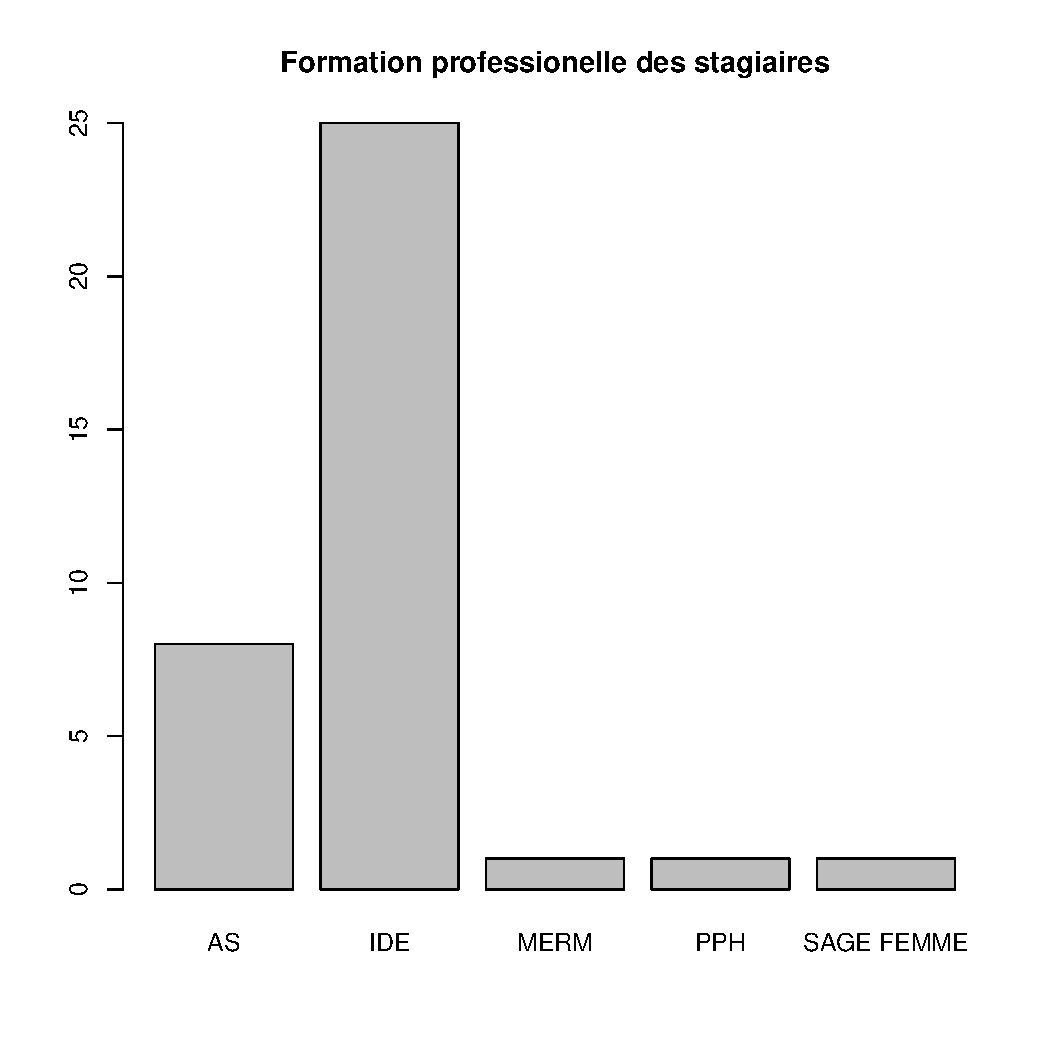
\includegraphics[width=\maxwidth]{figure/formation} 

\end{knitrout}


\subsection{expérience professionnelle}

Confrontation avec des situations d'urgence:
\begin{knitrout}
\definecolor{shadecolor}{rgb}{0.969, 0.969, 0.969}\color{fgcolor}\begin{kframe}
\begin{verbatim}
## non oui 
##  20  16
\end{verbatim}
\end{kframe}
\end{knitrout}





\section{Echelle de Likert}

Pour chaque item de l'echelle de Likert, on présente:
\begin{itemize}
  \item une représentation graphique de l'echelle avant/après
  \item une comparaison des deux moyennes au moyen du test t de Student pour séries appariées. Une différence entre les moyennes avant/après est considérée comme significative lorsque la probabilité d'observer une telle différence (p) est inférieure à $0.05$, c'est à dire trop petite pour que cette différence soit due au hasard.
\end{itemize}

Les réponses aux questions se font sur une échelle allant 1 à 8, ce qui impose une zone de "neutralité" quelque part entre 4 et 5 sans que l'on puisse donner une valeur précise puisque les unités sont entières. Par convention, les opinions négatives correspondent aux valeurs basses de l'échelle (et donc à gauche sur un axe croissant) alors que les opinions positives répondent aux valeurs les plus élevées de l'échelle (et donc à droite sur un axe croissant).

Il existe de nombreuses manières de représenter graphiquement une échelle de Likert. N.B. Robbins et coll. après une analyse critique des représentations possibles recommandent d'utiliser la méthode des graphiques en barre empilées divergentes \cite{1}.
La zone neutre coincide avec la ligne verticale zéro. Tous ceux qui sont plutôt d'accord sont représenté à droite du zéro et dans des tons bleus dont l'intensité croit avec l'accord. Ceux qui sont en désaccord avec la proposition figurent à gauche du zéro et dans des tons rouges d'intensité croissante. Les couleurs ont été choisies pour convenir aux personnes déficientes visuelles. Les réponses sont automatiquement ajustées par rapport à cette ligne de référence ce qui permet de mesurer visuellement l'évolution du groupe.

\subsection{Question Q1}



Avant (Q1A):
\begin{knitrout}
\definecolor{shadecolor}{rgb}{0.969, 0.969, 0.969}\color{fgcolor}\begin{kframe}
\begin{verbatim}
##    Min. 1st Qu.  Median    Mean 3rd Qu.    Max.    NA's 
##    1.00    5.00    5.00    5.49    6.00    7.00       1
\end{verbatim}
\end{kframe}
\end{knitrout}

\begin{enumerate}
  \item \textbf{Min}imum = 4: une partie des personnes ont une opinion plutôt négative sur la proposition.
  \item \textbf{1st. Qu}artile = 5: Le premier quartile (appelé aussi Q25) est à 5 ce qui signifie que 25\% des répondants ont une opinion négative ou neutre sur la proposition.
  \item \textbf{Mediane} = 5: la médiane (appelée aussi Q50) correspond au deuxième quartile, c'est à dire que 50\% des répondants ont une opinion négative ou neutre et 50\% ont une opinion positive ou neutre.
  \item \textbf{Mean} = $5.3$: la moyenne des réponses est égale à $5.3$. Les chiffres décimaux sont toujours délicats à interpréter avec des valeurs entières. La proximité de la moyenne et de la médiane est un indice en faveur de la normalité des valeurs. Si les valeurs sont normales (c'est à dire qu'elles se répartissent comme une courbe de Gauss), ont peut utiliser des tests statistiques paramétriques comme le test de Student pour comparer deux moyennes (dans le cas contraire il faudrait utiliser des tests non paramétriques).
  \item \textbf{3rd. Qu}artile = 6: le troisième quartile (appelé aussi Q75) est égal à 6. Le troisième quartile correspond à 75\% des réponses. L'intervalle interquartile (entre Q25 et Q75) est faible. Globalement on peut dire que les personnes interrrogées ont une opinion neutre à modérément favorable par rapport à la question mais l'enthousiasme est faible.
  \item \textbf{max}imum = 7: quelque personnes sont assez d'accord avec la proposition, mais personne n'a coché le score maximal.
\end{enumerate}

Après (Q1B):
\begin{knitrout}
\definecolor{shadecolor}{rgb}{0.969, 0.969, 0.969}\color{fgcolor}\begin{kframe}
\begin{verbatim}
##    Min. 1st Qu.  Median    Mean 3rd Qu.    Max. 
##    6.00    7.00    7.00    7.11    7.25    8.00
\end{verbatim}
\end{kframe}
\end{knitrout}

Après la formation l'opinion du groupe à évoluée positivement. Toutes les opinions sont franchement favorables et personne ne se situe dans la zone de neutralité(\textbf{Min}imum = 6). Le score maximal est atteint (\textbf{max}imum = 8) et le troisième quartile (q75 = $7.5$) atteint presque le score maximal.

Graphiquement, cette évolution est bien visible (fig.\ref{Q1_likert}). La courbe des réponses se décale vers la droite tandis que les nuances de bleu se renforcent (Q1B) traduisant une forte augmentation des opinions positives.

Il y a une différence significative entre les moyennes des scores avant et après, que l'on peut objectiver avec un test de Student pour séries appariées. L'hypothèse neutre que l'on pose à priori est qu'il n'existe pas d'évolution dans l'opinion du groupe et que la différence avant/après est due au hasard. L'hypothèse alternative est qu'au contraire, il y a une évolution dans l'opinion du groupe. Le test statistique évalue l'hypothèse neutre  et le résultat obtenu amène à rejeter l'hypothèse neutre (la différence avant/après n'est pas due au hasard) et par conséquent d'accepter l'hypothèse alternative.

($t(34)=-7.125$,
$p < 0.001$).
(Voir figure \ref{Q1_box} page \pageref{Q1_box}).
La valeur p indique que l'on a moins d'une chance sur $1000$ de se tromper en affirmant que l'hypothèse neutre est fausse.

\begin{figure}
\begin{center}
\begin{knitrout}
\definecolor{shadecolor}{rgb}{0.969, 0.969, 0.969}\color{fgcolor}
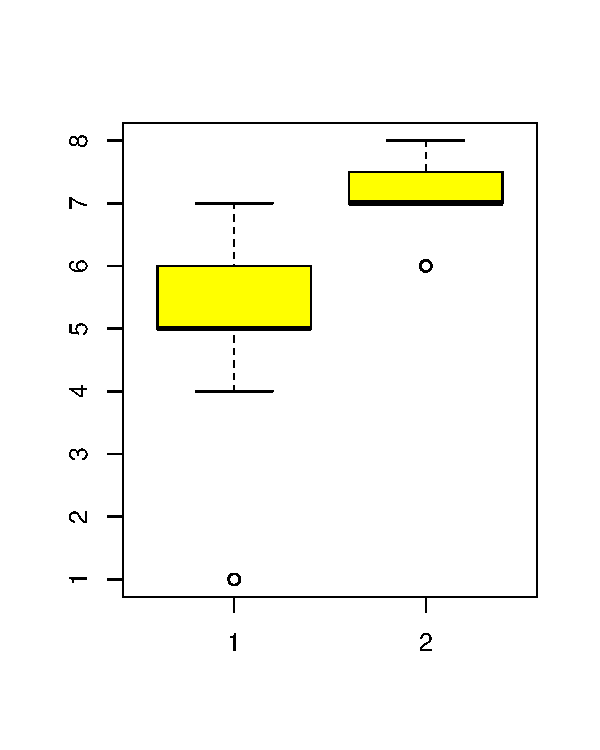
\includegraphics[width=\maxwidth]{figure/Q1_boxplot} 

\end{knitrout}

\end{center}
\caption{Représentation sous forme de "boite à moustaches" (box-plot) de l'évolution des opinions pour la question Q1 - Avant/Après. Les rectangles jaunes correspondent à la distance interquartile (Q25-Q75) et le trait épais à la médiane. On observe que non seulement les opinions ont évolués positivement mais que l'opinion du groupe est plus consensuelle (rectangle plus petit). L'absence de chevauchement des deux rectangles indique que la différence avant/après sera statistiquement significative.}
\label{Q1_box}
\end{figure}




\begin{figure}
\begin{center}
\begin{knitrout}
\definecolor{shadecolor}{rgb}{0.969, 0.969, 0.969}\color{fgcolor}
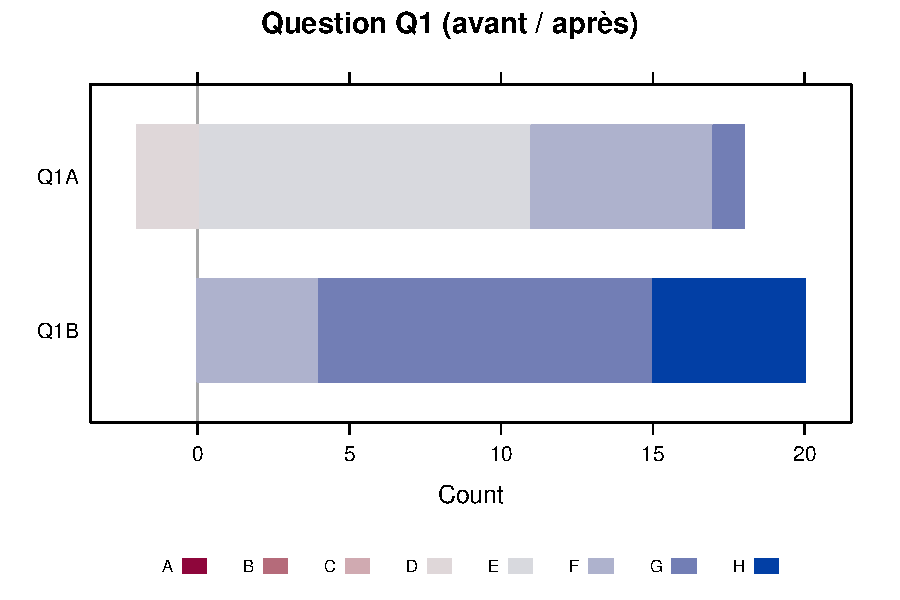
\includegraphics[width=\maxwidth]{figure/likert_Q1} 

\end{knitrout}

\end{center}
\caption{Evolution des opinions pour la question Q1 - Avant/Après. L'évolution fortement positive du groupe se traduit par un renforcement des nuances de bleu pour la question Q1B et le décalage de la courbe vers la droite. En abscisse figure la taille du groupe (count).}
\label{Q1_likert}
\end{figure}

%%%%%%%%%%%%%%%%%%%%%%%%%%%%%%%%%
\subsection{ Question Q4}
%%%%%%%%%%%%%%%%%%%%%%%%%%%%%%%%%

Question 4: \emph{je pense que n'hésite pas à prendre des décisions en situation d'urgence}

\begin{knitrout}
\definecolor{shadecolor}{rgb}{0.969, 0.969, 0.969}\color{fgcolor}
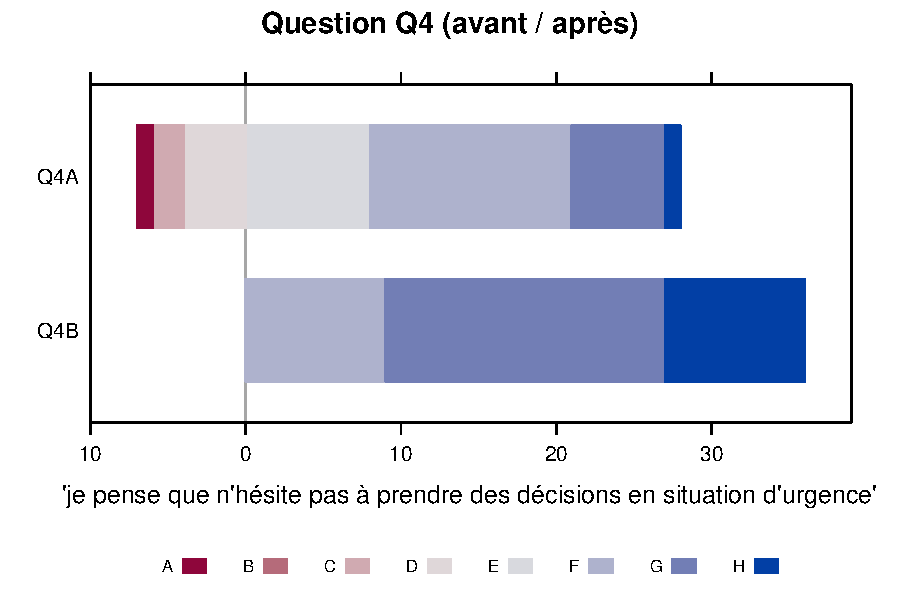
\includegraphics[width=\maxwidth]{figure/q4} 

\end{knitrout}

Avant la formation, une partie du groupe n'est pas d'accord avec la proposition (Q1A) ce qui peut s'interpréter comme un manque d'assurance face à ce type de situation. Après la formation, l'opinion du groupe se décale fortement sur la droite (Q1B) traduisant une augmentation importante de sa confiance en soi.

\begin{knitrout}
\definecolor{shadecolor}{rgb}{0.969, 0.969, 0.969}\color{fgcolor}\begin{kframe}
\begin{verbatim}
##    1    3    4    5    6    7    8 NA's 
##    1    2    4    8   13    6    1    1
##  6  7  8 
##  9 18  9
\end{verbatim}
\end{kframe}
\end{knitrout}



%%%%%%%%%%%%%%%%%%%%%%%%%%%%%%%%%
\subsection{ Question Q6}
%%%%%%%%%%%%%%%%%%%%%%%%%%%%%%%%%
question 6: \emph{Même en situation d'urgence je préfère attendre un collègue}

\begin{knitrout}
\definecolor{shadecolor}{rgb}{0.969, 0.969, 0.969}\color{fgcolor}
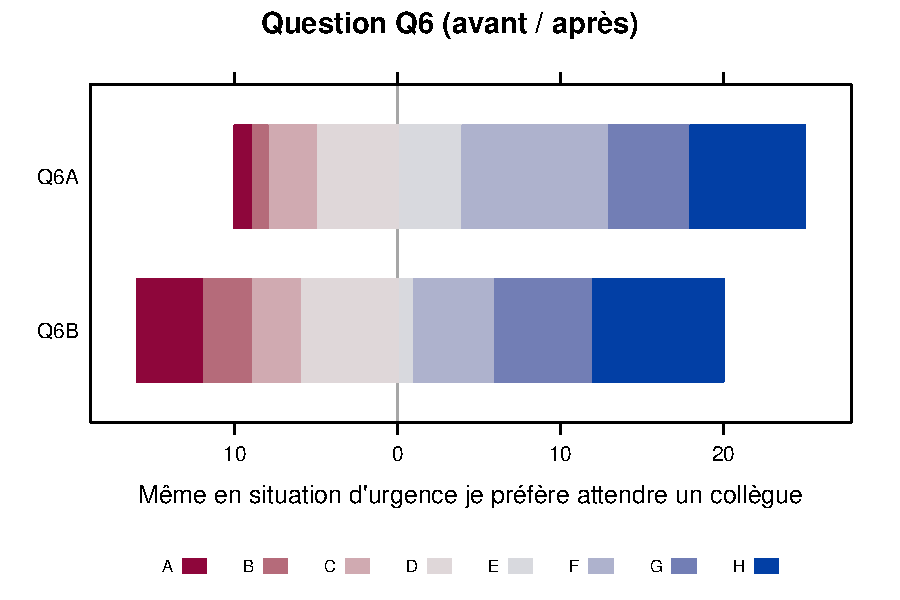
\includegraphics[width=\maxwidth]{figure/q6} 

\end{knitrout}


Cette question est à l'opposé de la question 4. Il est donc normal qu'une partie importante du groupe soit en désaccord avec cette proposition. Après la formation, la position des apprenants évolue vers un renforcement des opinions négatives ce qui est cohérent, mais cette évolution est moins marquée que pour la question 4. Ainsi à l'issue de la formation, les apprenants sont plus enclins à prendre des décisions en situation d'urgence mais l'aval d'un pair reste important.

\begin{knitrout}
\definecolor{shadecolor}{rgb}{0.969, 0.969, 0.969}\color{fgcolor}\begin{kframe}
\begin{verbatim}
##    1    2    3    4    5    6    7    8 NA's 
##    1    1    3    5    4    9    5    7    1
## 1 2 3 4 5 6 7 8 
## 4 3 3 6 1 5 6 8
\end{verbatim}
\end{kframe}
\end{knitrout}


%%%%%%%%%%%%%%%%%%%%%%%%%%%%%%%%%%%%%%%%%%%%%%%%%%%
\section{Sentiment d'efficacité personnelle (SEP)}
%%%%%%%%%%%%%%%%%%%%%%%%%%%%%%%%%%%%%%%%%%%%%%%%%%%

A l'aide des questions Q1 à Q9 on construit une échelle composite répondant aux critères d'une échelle de Likert. En pratique deux échelles sont construites à partir des mêmes items mesurés avant at après la formation. Chaque échelle réalise la somme non pondérée de chaque item.
\begin{knitrout}
\definecolor{shadecolor}{rgb}{0.969, 0.969, 0.969}\color{fgcolor}\begin{kframe}
\begin{verbatim}
##  [1] 44 48 49 55 45 45 51 56 47 52 49 50 45 43 44 63 46 58 53 39 50 63 55
## [24] 56 58 47 57 40 23 58 NA 60 61 54 55 37
##    Min. 1st Qu.  Median    Mean 3rd Qu.    Max.    NA's 
##    23.0    45.0    50.0    50.2    56.0    63.0       1
\end{verbatim}
\end{kframe}
\end{knitrout}

On répète l'opération pour les mesures après:
\begin{knitrout}
\definecolor{shadecolor}{rgb}{0.969, 0.969, 0.969}\color{fgcolor}\begin{kframe}
\begin{verbatim}
##    Min. 1st Qu.  Median    Mean 3rd Qu.    Max. 
##    51.0    58.0    61.0    61.2    64.0    72.0
\end{verbatim}
\end{kframe}
\end{knitrout}


Globalement le SEP augmente entre le début et la fin de la formation. Le graphe montre également une plus grande cohérence du groupe en fin de formation (resserrement autour de la moyenne).
\begin{knitrout}
\definecolor{shadecolor}{rgb}{0.969, 0.969, 0.969}\color{fgcolor}
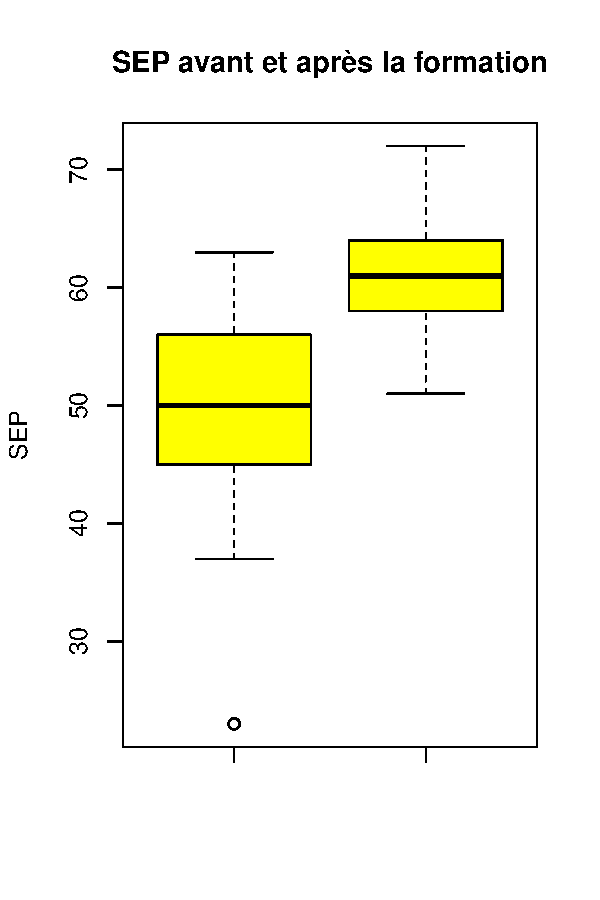
\includegraphics[width=\maxwidth]{figure/sepboxplot} 

\end{knitrout}

Et cette évolution est très significative:
\begin{knitrout}
\definecolor{shadecolor}{rgb}{0.969, 0.969, 0.969}\color{fgcolor}\begin{kframe}
\begin{verbatim}
## 
## 	Welch Two Sample t-test
## 
## data:  a and b 
## t = -6.843, df = 54.13, p-value = 7.339e-09
## alternative hypothesis: true difference in means is not equal to 0 
## 95 percent confidence interval:
##  -14.253  -7.794 
## sample estimates:
## mean of x mean of y 
##     50.17     61.19
\end{verbatim}
\end{kframe}
\end{knitrout}

($t(54.1264)=-6.843$,
$p < 0.001$).


L'étude de la différence sepb - sepa montre que si globalement le SEP augmente après la formation (moyenne de 11 points), il régresse pour certains (-4) et augmente massivement pour d'autres (+42):
\begin{knitrout}
\definecolor{shadecolor}{rgb}{0.969, 0.969, 0.969}\color{fgcolor}\begin{kframe}
\begin{verbatim}
##    Min. 1st Qu.  Median    Mean 3rd Qu.    Max.    NA's 
##    -4.0     6.0    10.0    11.1    16.5    42.0       1
##  [1] 14 16 15  6 18 12 14 11 19  8 10  6  6 13 17 -4  9  2  9 19 19 -1  0
## [24]  7  1 24  1 20 42  7 NA  4 11 -2  9 25
\end{verbatim}
\end{kframe}
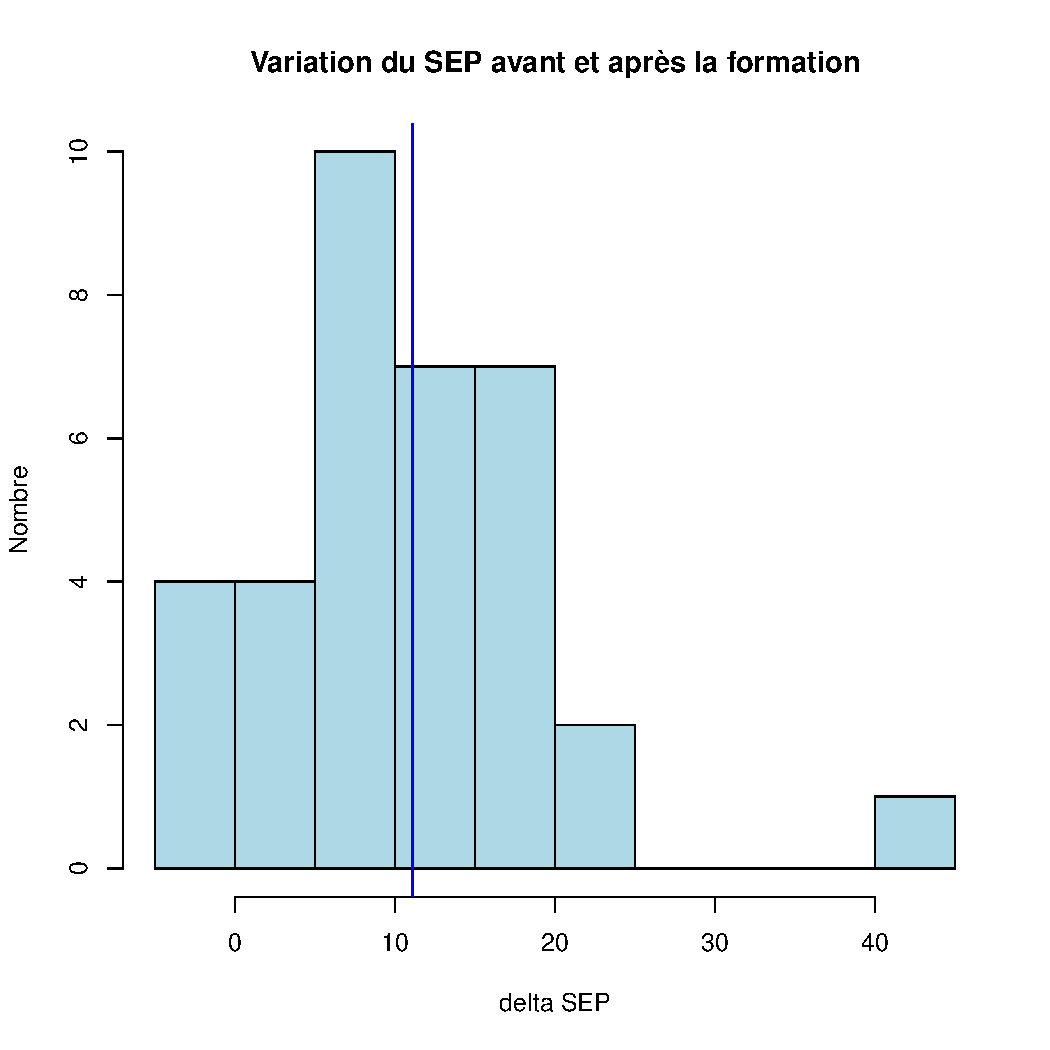
\includegraphics[width=\maxwidth]{figure/sep9a-b} 

\end{knitrout}

La progression la plus spectaculaire est observée pour un préparateur en pharmacie. En moyenne la progression par groupe socio-professionnel s'établit ainsi:
\begin{knitrout}
\definecolor{shadecolor}{rgb}{0.969, 0.969, 0.969}\color{fgcolor}\begin{kframe}
\begin{verbatim}
##       MERM         AS        IDE SAGE FEMME        PPH 
##       7.00       7.29      10.76      18.00      42.00
\end{verbatim}
\end{kframe}
\end{knitrout}


\subsection{SEP et expérience des situations d'urgence}
%%%%%%%%%%%%%%%%%%%%%%%%%%%%%%%%%
SEP moyen en fonction de l'expérience:
\begin{knitrout}
\definecolor{shadecolor}{rgb}{0.969, 0.969, 0.969}\color{fgcolor}\begin{kframe}
\begin{verbatim}
##   non   oui 
## 47.58 53.25
\end{verbatim}
\end{kframe}
\end{knitrout}

Le SEP moyen est plus élevé chez ceux qui ont déjà connu des situations d'urgence.

\subsection{SEP et fréquence des situations d'urgence}
%%%%%%%%%%%%%%%%%%%%%%%%%%%%%%%%%%%%%%%%%%%%%%%%%%%%%%
\begin{knitrout}
\definecolor{shadecolor}{rgb}{0.969, 0.969, 0.969}\color{fgcolor}\begin{kframe}
\begin{verbatim}
##   jamais rarement  parfois  souvent 
##    39.20    48.20    52.05    55.60
\end{verbatim}
\end{kframe}
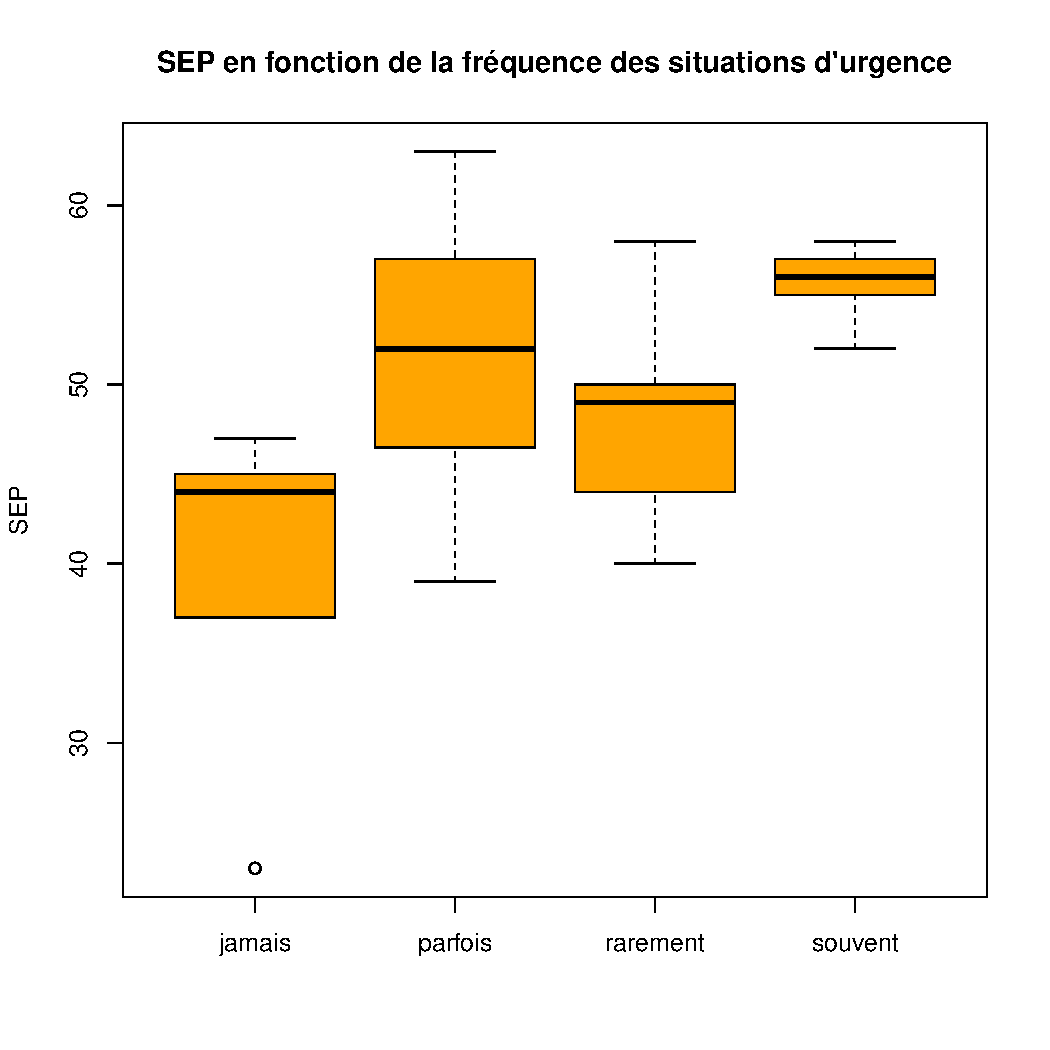
\includegraphics[width=\maxwidth]{figure/sepexp1} 
\begin{kframe}\begin{verbatim}
## Call:
##    aov(formula = a ~ conf_urg)
## 
## Terms:
##                 conf_urg Residuals
## Sum of Squares     839.2    1491.8
## Deg. of Freedom        3        31
## 
## Residual standard error: 6.937 
## Estimated effects may be unbalanced
## 1 observation deleted due to missingness
##             Df Sum Sq Mean Sq F value Pr(>F)   
## conf_urg     3    839   279.7    5.81 0.0028 **
## Residuals   31   1492    48.1                  
## ---
## Signif. codes:  0 '***' 0.001 '**' 0.01 '*' 0.05 '.' 0.1 ' ' 1 
## 1 observation deleted due to missingness
\end{verbatim}
\end{kframe}
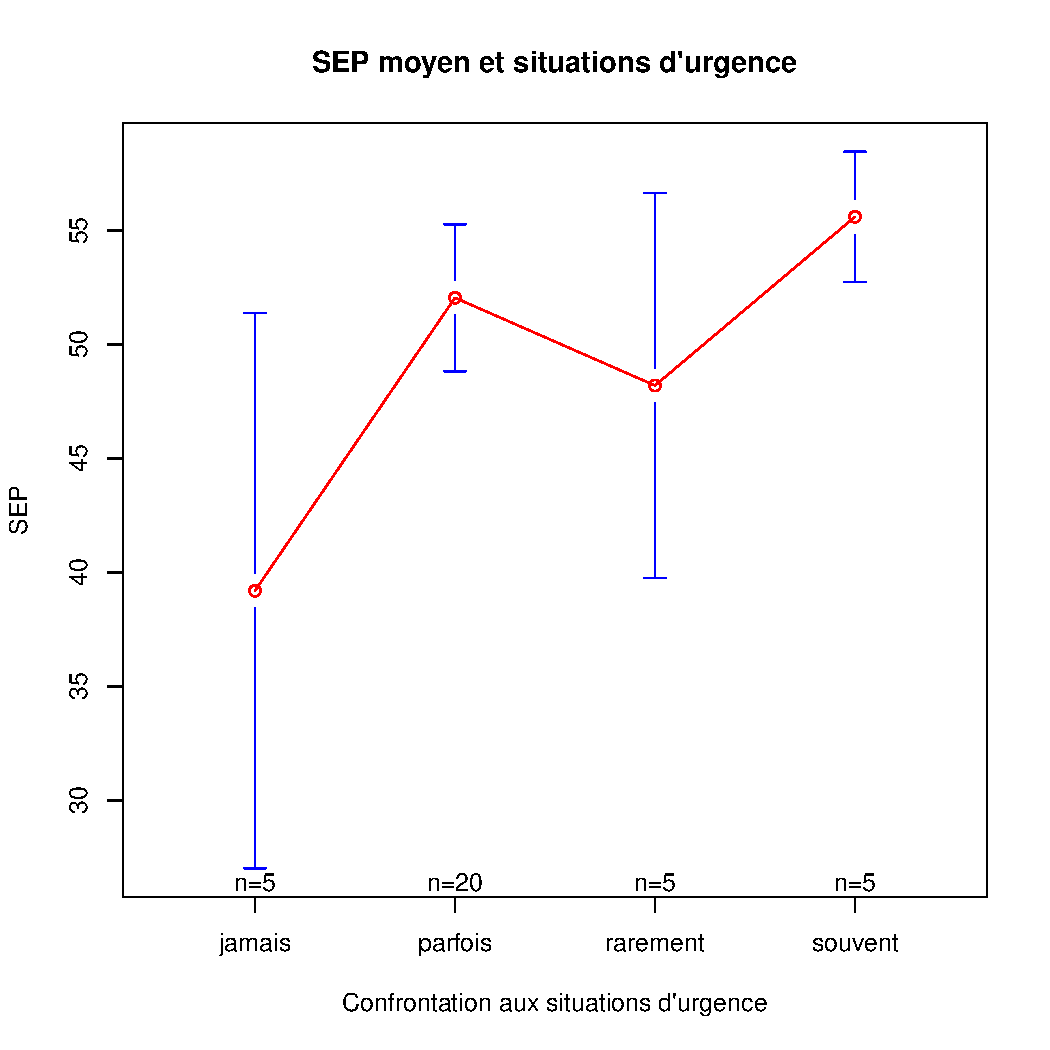
\includegraphics[width=\maxwidth]{figure/sepexp2} 
\begin{kframe}\begin{verbatim}
##   Tukey multiple comparisons of means
##     95% family-wise confidence level
## 
## Fit: aov(formula = a ~ conf_urg)
## 
## $conf_urg
##                   diff     lwr    upr  p adj
## parfois-jamais   12.85   3.436 22.264 0.0043
## rarement-jamais   9.00  -2.907 20.907 0.1916
## souvent-jamais   16.40   4.493 28.307 0.0040
## rarement-parfois -3.85 -13.264  5.564 0.6862
## souvent-parfois   3.55  -5.864 12.964 0.7371
## souvent-rarement  7.40  -4.507 19.307 0.3476
\end{verbatim}
\end{kframe}
\end{knitrout}



%%%%%%%%%%%%%%%%%%
% fin du document
%%%%%%%%%%%%%%%%%%

\bibliographystyle{plain} 
\bibliography{biblio}
\end{document}
